% Source of the figure PDF (pdflatex). Fonts match the paper: Times text (IEEEtran ptm), CM math, 10pt sizes.
\documentclass[10pt,border=0pt]{standalone}
\usepackage{times}
\usepackage{amsmath,amssymb}
\usepackage{xcolor}
\usepackage{tikz}
\usetikzlibrary{arrows.meta,positioning,shapes.geometric,calc,fit,backgrounds}
% same text settings as IEEEtran.cls (hyphenation penalty, badness, no extra space after punctuation)
\hyphenpenalty=750
\hbadness=1350
\frenchspacing
\usepackage{pgfplots}
\pgfplotsset{compat=1.17}
\begin{document}
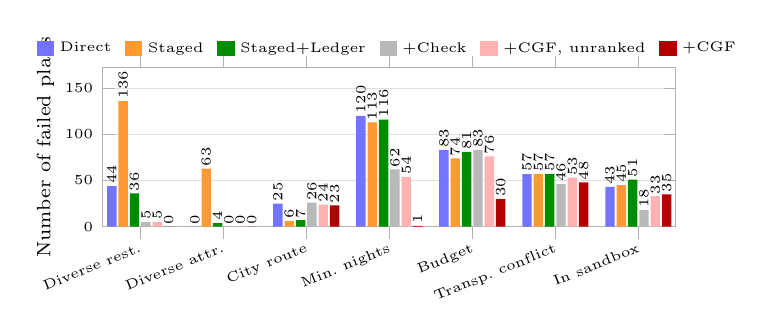
\begin{tikzpicture}
\begin{axis}[
  ybar=0.7pt, bar width=3.4pt, width=252pt, height=3.6cm,
  enlarge x limits=0.075, ymin=0, ymax=172,
  symbolic x coords={rest,attr,route,nights,budget,transp,sandbox},
  xtick=data,
  xticklabels={Diverse rest.,Diverse attr.,City route,Min.\ nights,Budget,Transp.\ conflict,In sandbox},
  x tick label style={font=\tiny, rotate=22, anchor=north east, inner sep=1pt},
  ytick={0,50,100,150}, y tick label style={font=\tiny}, /pgf/number format/assume math mode=true,
  ylabel={Number of failed plans}, ylabel style={font=\scriptsize, yshift=-3pt},
  nodes near coords, every node near coord/.append style={font=\fontsize{4.5}{5}\selectfont, rotate=90, anchor=west, inner sep=0.6pt, black},
  legend style={font=\tiny, at={(0.5,1.0)}, anchor=south, legend columns=6, draw=none, fill=none, /tikz/every even column/.append style={column sep=3pt}},
  legend image code/.code={\draw[#1, draw=none] (0cm,-0.08cm) rectangle (0.22cm,0.1cm);},
  ymajorgrids, grid style={gray!25}, axis line style={gray!60}, tick style={gray!60}
]
\addplot[fill=blue!55, draw=none] coordinates {(rest,44) (attr,0) (route,25) (nights,120) (budget,83) (transp,57) (sandbox,43)};
\addplot[fill=orange!80, draw=none] coordinates {(rest,136) (attr,63) (route,6) (nights,113) (budget,74) (transp,57) (sandbox,45)};
\addplot[fill=green!55!black, draw=none] coordinates {(rest,36) (attr,4) (route,7) (nights,116) (budget,81) (transp,57) (sandbox,51)};
\addplot[fill=gray!55, draw=none] coordinates {(rest,5) (attr,0) (route,26) (nights,62) (budget,83) (transp,46) (sandbox,18)};
\addplot[fill=red!30, draw=none] coordinates {(rest,5) (attr,0) (route,24) (nights,54) (budget,76) (transp,53) (sandbox,33)};
\addplot[fill=red!70!black, draw=none] coordinates {(rest,0) (attr,0) (route,23) (nights,1) (budget,30) (transp,48) (sandbox,35)};
\legend{Direct, Staged, Staged+Ledger, +Check, {+CGF, unranked}, +CGF}
\end{axis}
\end{tikzpicture}
\end{document}
